\documentclass[14pt, a4paper]{article}
\usepackage[russian]{babel}
\usepackage{graphicx}
% \usepackage{tabularx}
\usepackage{layout}
\usepackage[14pt]{extsizes}
\usepackage[hidelinks]{hyperref}
\usepackage{caption}

\usepackage{listings}
\usepackage{xcolor}

% \usepackage[compact]{titlesec}


\setlength{\emergencystretch}{5pt}


% 12/14pt


\definecolor{codegreen}{rgb}{0,0.6,0}
\definecolor{codegray}{rgb}{0.5,0.5,0.5}
\definecolor{codepurple}{rgb}{0.58,0,0.82}
\definecolor{backcolour}{rgb}{0.97,0.97,0.97}

\lstdefinestyle{mystyle}{
    backgroundcolor=\color{backcolour},   
    commentstyle=\color{codegreen},
    keywordstyle=\color{magenta},
    numberstyle=\tiny\color{codegray},
    stringstyle=\color{codepurple},
    basicstyle=\ttfamily\footnotesize,
    breakatwhitespace=false,         
    breaklines=true,                 
    captionpos=b,                    
    keepspaces=true,
    frame=single,                 
    % numbers=left,                    
    % numbersep=5pt,                  
    showspaces=false,                
    showstringspaces=false,
    showtabs=false,                  
    tabsize=2
}

\lstset{style=mystyle}


\oddsidemargin = 0pt
\marginparwidth = 45pt %57
\textwidth = 467pt
\textheight = 716pt
\topmargin = 0pt %17
\footskip = 30pt %30
\headheight = 0pt %12
\headsep = 0pt %25


\title{Методичка 4}

\begin{document}

\begin{titlepage}
    \topmargin=216pt
    \newpage
    \hangindent=0.7cm
    \huge ИУ-10\\
    Системное\\
    Программное\\
    Обеспечение\\
    \textbf{Системы виртуализации\\ Гипервизоры первого типа\\
    (baremetal hypervisors)}

    \vspace{10cm}

    \begin{center}
        \small\textit{Москва, 2022}
    \end{center}
\end{titlepage}
% \layout ##########################################################################################
\section*{На этом уроке}
\begin{enumerate}
    \item Рассмотрим общие особенности гипервизоров первого типа.
    \item Познакомимся с одним из самых широко используемых в корпоративной среде гипервизоров
    — VMware ESXi.
\end{enumerate}
\tableofcontents
\newpage

\section*{Общие особенности}
\addcontentsline{toc}{section}{Общие особенности}

\subsection*{Высокая эффективность и работа с аппаратурой}
\addcontentsline{toc}{subsection}{Высокая эффективность и работа с аппаратурой}

Виртуализация больших вычислительных машин, mainframe IBM, была реализована в далёких
60–70-х годах прошлого столетия. В те времена ещё не существовало мощных и универсальных
операционных систем общего назначения. Уже была в меру популярная ОС Multics, в противовес
которой позже будет разработана и поныне существующая ОС Unix. Тем не менее инженеры
компании IBM были недовольны реализацией многозадачности в Multics и пошли своим путём,
реализовав первый гипервизор. Разумеется, гипервизор работал непосредственно на «голом железе»
(англ. bare metal), то есть код гипервизора выполнялся напрямую процессором и гипервизор не
полагался на ОС или какое-либо другое ПО. Поскольку такова была реализация первого в мире
гипервизора, она получила название «гипервизор первого типа».

На рисунке ниже показана в упрощённом виде система с гипервизором первого типа:

\begin{figure}[h]%current location
    \centering
    \scalebox{1}{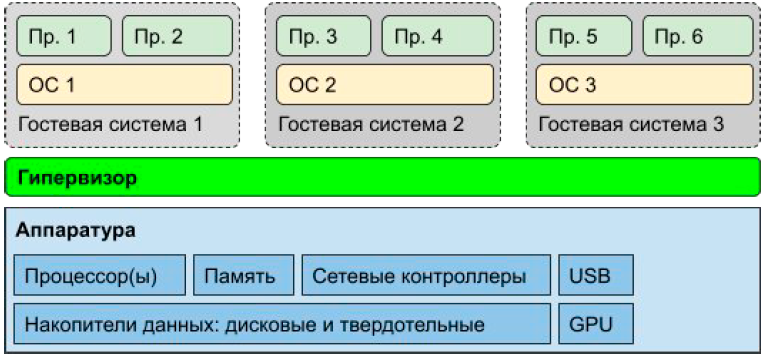
\includegraphics[width=1\textwidth]{imgs/1.1.png}}
    % \caption*{\textit{Выполнение ПО в разных режимах работы процессора}}
    \label{framework} %framework,fig1
\end{figure}

Глядя на рисунок, можно представить, что между аппаратурой и гостевыми системами существует
гипервизор в виде обязательной прослойки. Однако стоит иметь в виду, что это очень упрощённое
представление, потому как в современных системах гипервизор в первую очередь настраивает
виртуальное окружение для гостевой системы. Затем он относительно редко вступает в работу, давая
возможность гостевой системе работать самостоятельно, в том числе взаимодействовать
непосредственно с аппаратурой. Именно благодаря этому достигается высокая эффективность
системы в целом. Тем не менее изображённая выше модель позволяет визуализировать различия
между гипервизорами первого и второго типа. Для удобства сравнения на рисунке ниже показана
упрощённая модель системы с гипервизором второго типа:

\begin{figure}[h]%current location
    \centering
    \scalebox{1}{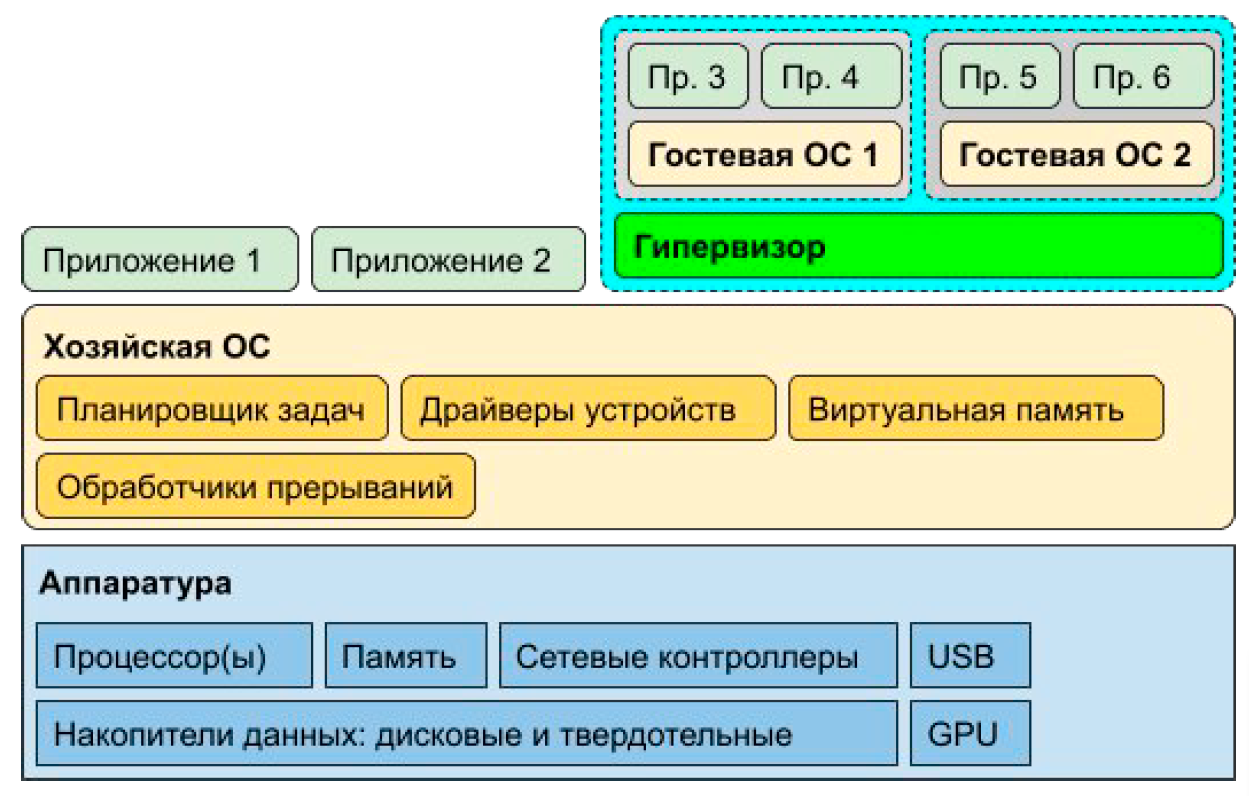
\includegraphics[width=1\textwidth]{imgs/1.2.png}}
    % \caption*{\textit{Выполнение ПО в разных режимах работы процессора}}
    \label{framework} %framework,fig1
\end{figure}

По сути, в случае гипервизора первого типа роль ОС выполняет сам гипервизор. В частности,
гипервизор инициализирует и настраивает аппаратуру, занимается распределением и учётом
ресурсов, таких как процессорное время и память, обрабатывает исключительные ситуации,
вызванные сбоями в работе аппаратуры или ПО. Кроме того, необходимо ещё обеспечить способ
взаимодействия пользователя с гипервизором, то есть нужен некий интерфейс пользователя:
командная строка, веб-интерфейс или что-то ещё.

Как мы знаем, удобство использования ОС, в частности, состоит в том, что современные ОС общего
назначения имеют развитую поддержку огромного парка оборудования. Это касается и центральных
процессоров, и разнообразных периферийных устройств. Отказываясь от использования ОС,
разработчик гипервизора вынужден обеспечивать поддержку интересного ему оборудования своими
силами. Резонно предположить, что разработчики такого узкоспециализированного ПО, как
гипервизоры, вряд ли имеют достаточно ресурсов и времени, чтобы поддерживать огромный парк
аппаратуры хоть сколько-то близко к ОС общего назначения. А потому разработчики вынуждены идти
одним из двух путей: обеспечить поддержку сильно ограниченного перечня аппаратуры или всё-таки
использовать ОС для предоставления определённых сервисов. В частности, ОС обеспечивают работу
с реальными устройствами при помощи имеющихся драйверов, а также реализуют богатый
функциональностью интерфейс пользователя.

Первый путь выбрали инженеры компании VMware для своего гипервизора ESXi. Они реализовали
замечательный пример монолитного гипервизора первого типа в исконном понимании этого термина,
которое изложили Попек и Голдберг в своей работе Formal Requirements for Virtualizable Third
Generation Architectures.

\begin{figure}[h]%current location
    \centering
    \scalebox{0.7}{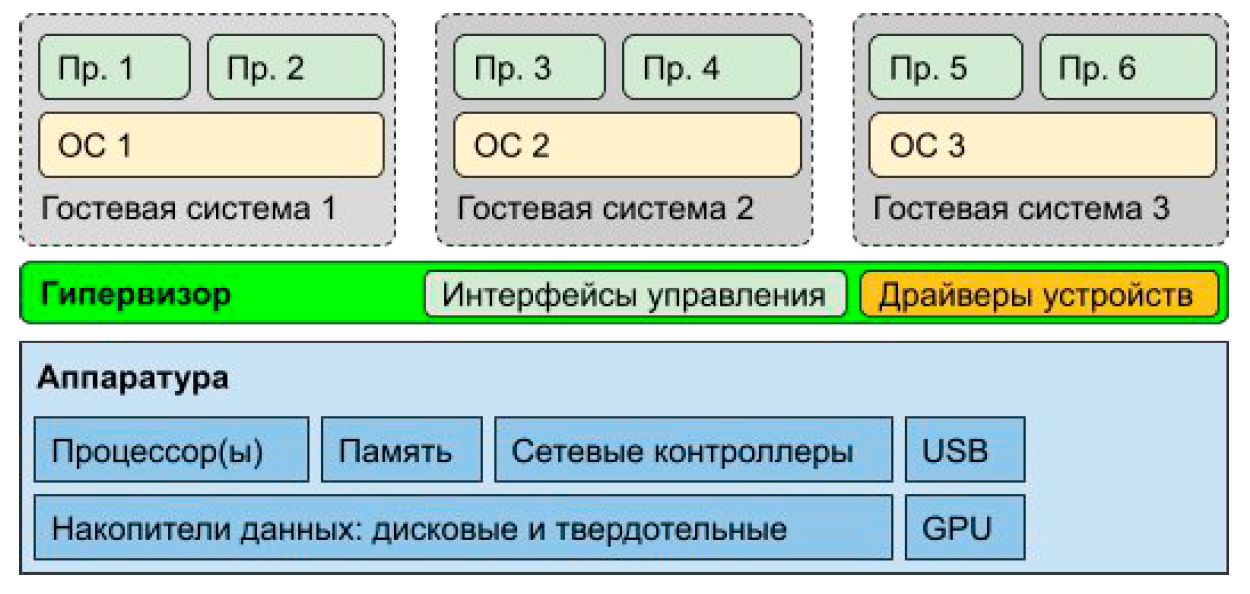
\includegraphics[width=1\textwidth]{imgs/1.3.png}}
    % \caption*{\textit{Выполнение ПО в разных режимах работы процессора}}
    \label{framework} %framework,fig1
\end{figure}

Гипервизор VMware ESXi устанавливается так, как будто это ещё одна ОС общего назначения, и
после установки он может работать совершенно самодостаточно, пусть и бесцельно. Если
пользователь настроил запуск каких-то гостевых систем, то они могут быть запущены автоматически
или по команде.

Разработчики Microsoft Hyper-V и Xen Hypervisor избрали вариант микроядерного гипервизора.
Схематично систему с микроядерным гипервизором можно изобразить следующим образом:

\begin{figure}[h]%current location
    \centering
    \scalebox{0.7}{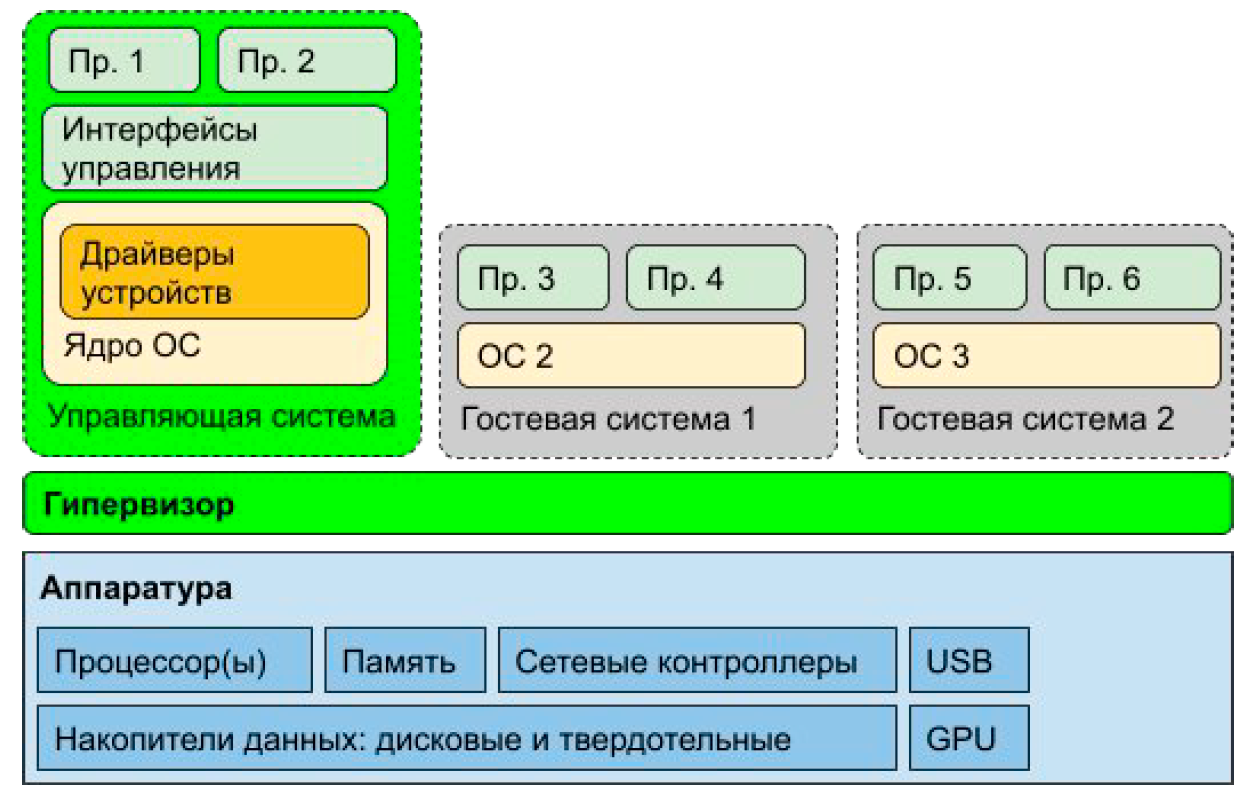
\includegraphics[width=1\textwidth]{imgs/1.4.png}}
    % \caption*{\textit{Выполнение ПО в разных режимах работы процессора}}
    \label{framework} %framework,fig1
\end{figure}

Гипервизор, имея в своем составе достаточно минималистичных драйверов для инициализации
процессора и накопителя данных, загружает в память и запускает первую виртуальную машину с
управляющей системой. А далее, при необходимости, управляющая система стартует прочие
виртуальные машины.

Разработчики KVM выбрали средний путь: роль гипервизора выполняет модуль ядра ОС Linux. Таким
образом, управляющая система — это обыкновенный, основанный на ядре Linux, дистрибутив
(Ubuntu, Debian, Red Hat, CentOS и далее, на вкус читателя), совместно с которым могут быть
запущены другие ОС в виртуальных окружениях.

\begin{figure}[h]%current location
    \centering
    \scalebox{0.7}{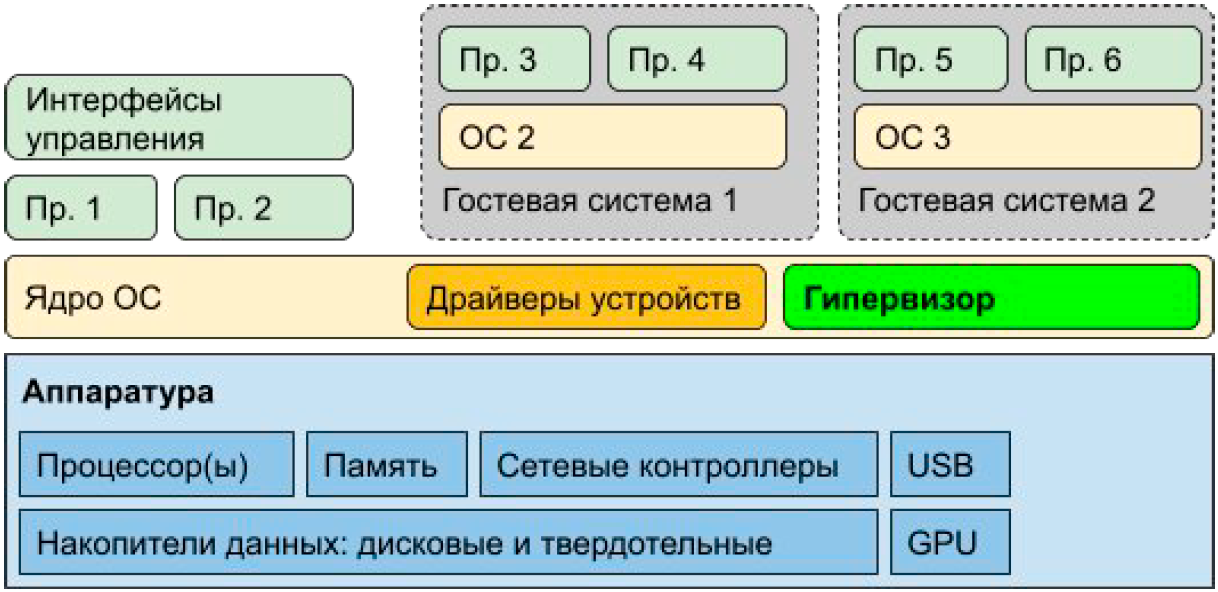
\includegraphics[width=1\textwidth]{imgs/1.5.png}}
    % \caption*{\textit{Выполнение ПО в разных режимах работы процессора}}
    \label{framework} %framework,fig1
\end{figure}

У каждого из решений есть свои преимущества и недостатки, но все их объединяет важное общее
преимущество перед гипервизорами, запущенными поверх хозяйской ОС: гипервизоры первого типа
изначально работают «ближе» к аппаратуре, а потому они оказываются более эффективными. Говоря
«ближе», мы имеем в виду, что гипервизор не пользуется сервисами ОС для работы с аппаратурой, а
самостоятельно ею управляет. Устранение дополнительного уровня абстракции позволяет сэкономить
ценное процессорное время для гостевых систем.

Именно благодаря этому гипервизоры первого типа позволяют гостевым системам работать почти так
же быстро, как если бы они были запущены непосредственно на аппаратуре. Это наглядно
показывают результаты измерений, которые уже приводились на предыдущем занятии, но мы ещё раз
обратимся к ним. Задачи, связанные с высокими вычислительными нагрузками (такие, как компиляция
ПО), хоть и незначительно, но быстрее выполняются гипервизорами первого типа. А вот задачи,
требующие создания множества процессов, выполняются существенно быстрее гипервизорами
первого типа, при этом они весьма близки к производительности реальной системы без гипервизора.
Мы можем убедиться в правильности сделанных ранее предположений, основанных на анализе
устройства гипервизоров разного типа.

\begin{figure}[h]%current location
    \centering
    \scalebox{1}{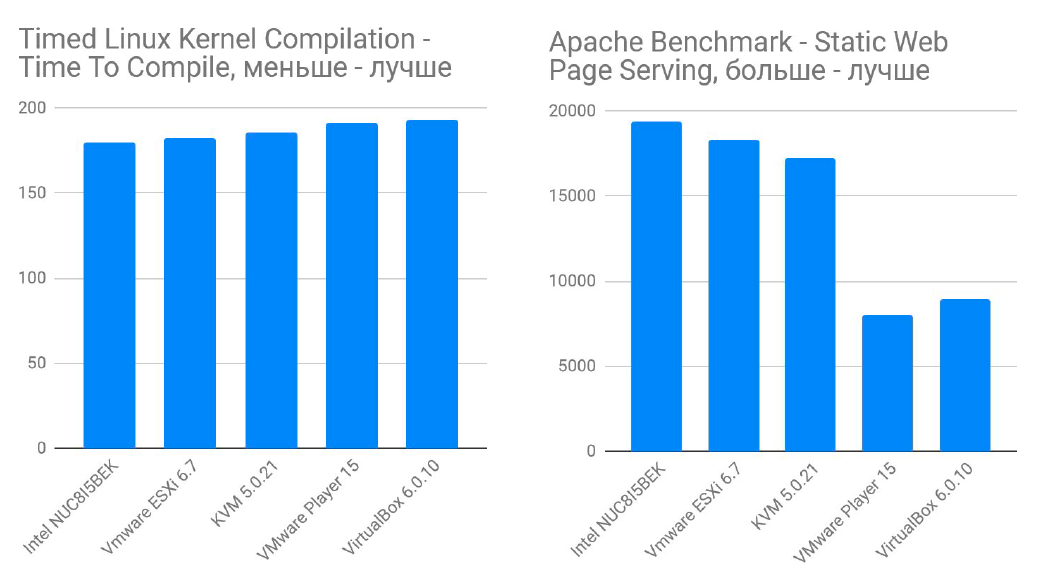
\includegraphics[width=1\textwidth]{imgs/1.6.png}}
    % \caption*{\textit{Выполнение ПО в разных режимах работы процессора}}
    \label{framework} %framework,fig1
\end{figure}

До сих пор мы рассматривали эффективность работы гипервизоров при запуске только одной
гостевой системы, а это достаточно редкая ситуация — во всяком случае, для серверной
виртуализации. Мы же помним, что одной из причин возникновения и широкого распространения
серверной виртуализации была и остаётся возможность более эффективного использования
имеющихся аппаратных ресурсов за счёт запуска нескольких виртуальных систем на одном
экземпляре аппаратуры.

При запуске нескольких гостевых систем результаты могут оказаться другими. Однако при выборе
гипервизора стоит произвести измерения в условиях, максимально близких к рабочим, и уже тогда
делать вывод о том, какая технология виртуализации показывает максимальную эффективность.

Справедливости ради стоит отметить, что не всегда есть возможность выбрать систему
виртуализации, особенно если приходится иметь дело с уже развёрнутой инфраструктурой. Даже
когда встаёт вопрос выбора, производительность или эффективность гипервизора может оказаться
второстепенным фактором на фоне вопросов, связанных со стоимостью владения системой, опытом
команды инженеров, имеющейся аппаратурой или требованиями заказчика.\\

\subsection*{Использование виртуальных машин в вычислительном кластере}
\addcontentsline{toc}{subsection}{Использование виртуальных машин в вычислительном кластере}

Выше мы рассмотрели два важных аспекта работы гипервизоров первого типа: их высокую
производительность относительно гипервизоров второго типа, а также особенности работы с
аппаратурой. Но использование гипервизора на одной отдельно взятой машине — это весьма редкий
случай, особенно для гипервизоров первого типа. Гораздо чаще используется несколько физических
серверов с гипервизорами, объединёнными в систему, которая используется как единый,
унифицированный компьютерный ресурс. Такую систему принято называть кластером. В самом
простом случае можно рассматривать кластер как совокупность физических серверов, гипервизоров и
виртуальных машин, запущенных поверх них.

\begin{figure}[h]%current location
    \centering
    \scalebox{1}{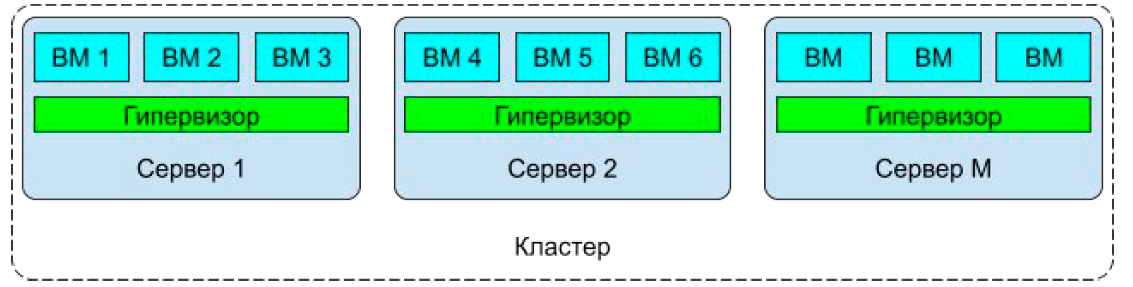
\includegraphics[width=1\textwidth]{imgs/1.7.png}}
    \label{framework} %framework,fig1
\end{figure}

Таким образом, вместо одного сервера с N виртуальных машин в нашем распоряжении оказывается в
M раз больше ресурсов и виртуальных машин. Мы исходим из того, что используется гомогенная
архитектура — одинаковые серверы с одинаково сконфигурированными гипервизорами. И несмотря
на то, что это выглядит наивным упрощением, на практике такой подход весьма оправдан и
рекомендуется к использованию, потому что такие системы гораздо проще администрировать и
эксплуатировать.

Пока опустим вопросы управления кластером, распределения задач и работы со сбоями, будем
просто рассматривать кластер как абстракцию, содержащую некоторое количество однородных
вычислительных ресурсов. В общем случае вычислительные узлы могут использоваться и без
виртуальных машин, запущенных поверх аппаратуры, но именно использование виртуальных машин
наделяет кластер воистину чудесными возможностями. Можно полностью контролировать состояние
виртуальных машин:

\begin{itemize}
    \item создавать и уничтожать виртуальные машины по мере необходимости;
    \item переносить виртуальные машины с одной физической системы на другую;
    \item иметь полную копию работающей виртуальной машины, чтобы при неожиданном отказе
    работающей виртуальной машины или сервера, на котором она была запущена, восстановить
    виртуальную машину в близком к исходному состоянии на новом сервере.\\
\end{itemize}

\subsection*{Масштабирование виртуальных машин}
\addcontentsline{toc}{subsection}{Масштабирование виртуальных машин}

Самое простое применение вычислительного кластера с виртуальными машинами состоит в гибком
управлении мощностью, предоставляемой сервисами виртуальных машин. Допустим, мы оказываем
услуги почтового сервиса и изначально приходится обслуживать 10 пользователей. Со временем наш
почтовый сервис снискал популярность и пользователей стало 10 000. С новой нагрузкой исходная
ВМ уже не может справиться. Однако если вычислительные ресурсы кластера ещё не исчерпаны,
можно использовать два решения:

\begin{enumerate}
    \item Увеличить количество вычислительных ресурсов, доступное данной ВМ. Это называется
    вертикальным масштабированием виртуальной машины.
    \begin{figure}[h]%current location
        \scalebox{1}{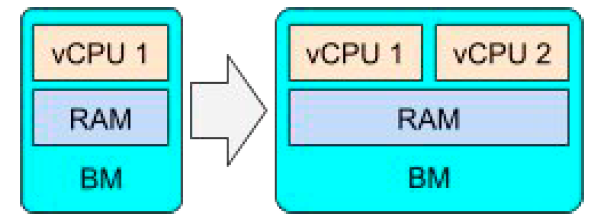
\includegraphics[width=0.5\textwidth]{imgs/1.8.png}}
        \label{1.8} %framework,fig1
    \end{figure}
    \item Увеличить количество используемых виртуальных машин. Это называется горизонтальным
    масштабированием виртуальных машин.
    \begin{figure}[h]%current location
        \scalebox{1}{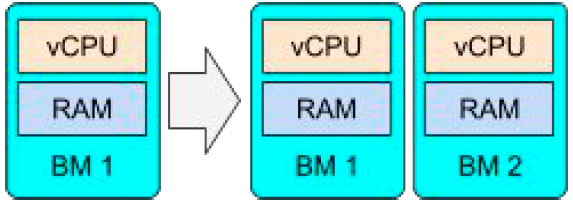
\includegraphics[width=0.5\textwidth]{imgs/1.9.png}}
        \label{1.9} %framework,fig1
    \end{figure}
\end{enumerate}

В случае снижения нагрузки возможно уменьшить количество выделенных виртуальной машине
ресурсов и/или остановить и удалить часть виртуальных машин, тем самым освободив
вычислительные ресурсы кластера под другие задачи. Современные системы управления
виртуальными машинами, кроме всего прочего, позволяют использовать автоматическое
масштабирование в ответ на изменяющуюся вычислительную нагрузку, тем самым обеспечивая ещё
большую эффективность и удобство использования вычислительных ресурсов. \\

\subsection*{Живая миграция виртуальных машин}
\addcontentsline{toc}{subsection}{Живая миграция виртуальных машин}

Перенос виртуальной машины, который ещё называют миграцией, происходит без остановки
виртуальной машины. Посмотрим, как же становится возможной миграция работающей виртуальной
машины.

Как мы обсуждали ранее, полное состояние виртуальной машины состоит из трёх сущностей:

\begin{enumerate}
    \item Данные на некой файловой системе. Это исполняемый код и данные, с которыми работает
    виртуальная машина, — обычно на некотором внешнем накопителе.
    \item Содержимое ОЗУ.
    \item Состояние процессора.
\end{enumerate}

Все три сущности уже доступны в удобном для сохранения и/или переноса виде. Внутри кластера
обычно используется файловая система, одинаково доступная для всех систем.

\begin{figure}[h]%current location
    \centering
    \scalebox{1}{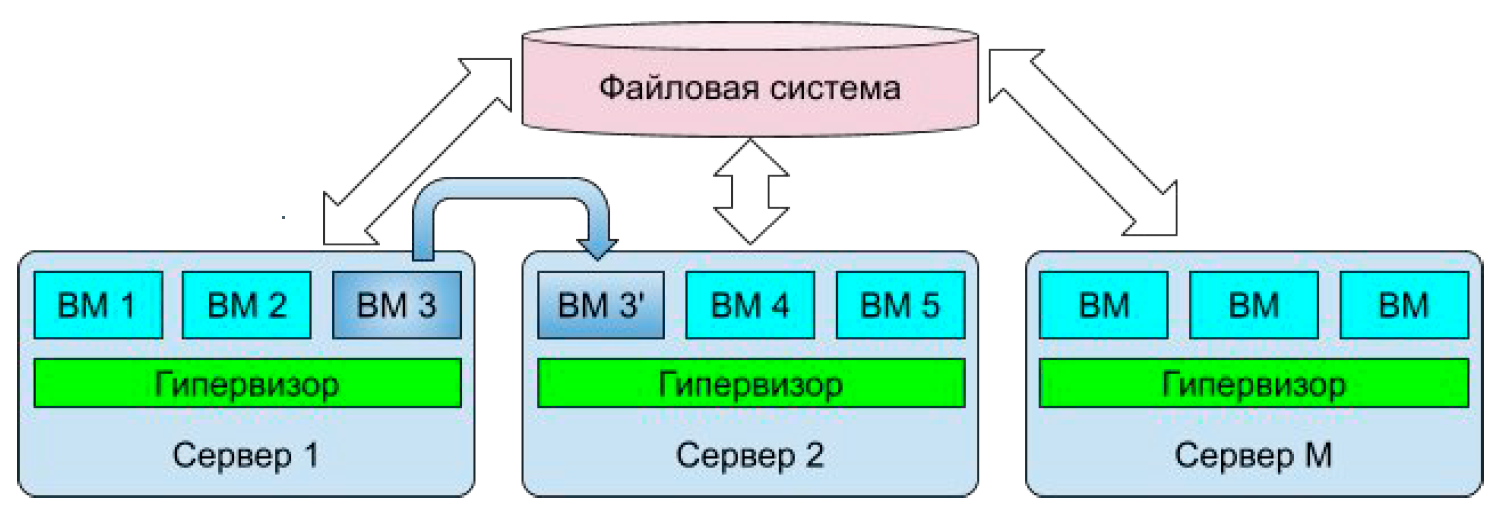
\includegraphics[width=1\textwidth]{imgs/1.10.png}}
    % \caption*{\textit{Выполнение ПО в разных режимах работы процессора}}
    \label{framework} %framework,fig1
\end{figure}

Это может быть распределённая файловая система, использующая накопители каждого из
физических серверов в кластере. Или, что встречается наиболее часто, централизованная сетевая
файловая система — такая как, например, NFS или iSCSI (читается «ай-скази»).

Гипервизор знает, какие страницы памяти используются каждой гостевой системой, а потому он может
получить доступ к их содержимому и либо сохранить содержимое памяти на файловую систему, либо
передать гипервизору другого сервера для восстановления образа памяти переносимой гостевой
системы. Такая же история и с состоянием виртуального процессора: оно изначально доступно
гипервизору и может быть также сохранено на файловой системе или передано другому гипервизору.

Думаем, вопросов насчёт равнодоступной всем серверам кластера файловой системы у вас не
возникает. Если её состояние изменяется, то эти изменения становятся доступны всем остальным
серверам, включая и тот, на который переносится гостевая система. С содержимым ОЗУ переносимой
системы всё не так очевидно, учитывая тот факт, что мы не хотим останавливать переносимую
систему — во всяком случае, на длительное время.

Если объём памяти, используемый гостевой системой, составляет десятки или даже сотни мегабайт,
то время, требующееся на копирование такого количества данных через современные гигабитные
сети, относительно мало. Действительно, 100 Мбайт в теории может быть передано через сеть 1 Гбит
за одну секунду. Речь идёт об идеальных условиях: без учёта затрат на метаданные, такие как
заголовки сетевых протоколов, управляющие сигналы и необходимость делить канал связи с другими
системами. Но для передачи десятков гигабайт данных может потребоваться значительное время,
измеряемое минутами.

Можно сделать предположение, что гостевая система не работает со всей доступной памятью
одновременно. Более того, часто бывает так, что в некотором промежутке времени реально
используется очень небольшое количество памяти. Во всяком случае, в хорошо написанном ПО
активно используется так называемая «локальность» памяти. Речь идёт о том, что плотно
сгруппированные команды и данные имеют шансы все сразу оказаться в кеше процессора или хотя
бы использовать ограниченное количество страниц памяти, обеспечивая максимальную скорость
обработки этих данных. Если же каждая следующая команда и блок данных оказывается вне
соответствующего кеша, и ещё для страницы с этой инструкцией или данными нет готовой трансляции
в MMU, выполнение такой программы будет феноменально неэффективным.

Можно сделать полную копию оперативной памяти всё ещё работающего гостя в фоновом режиме.
Фактически мы получим снимок состояния ОЗУ гостя в некоторый момент времени. И теперь остаётся
только отслеживать, какие новые изменения происходят в памяти всё ещё работающего гостя. Это
может быть легко сделано гипервизором: достаточно изменить флаги доступа всех страниц памяти
гостя на «доступна только для чтения» (англ. Read-only, RO). При попытке записи гостем данных в
любую страницу будет происходить исключение «страничного доступа», которое будет
перехватываться гипервизором. Гипервизор будет делать для себя отметку о том, что данная
страница была изменена с момента создания снимка, а затем изменять флаг доступа для данной
страницы на «доступна для чтения и записи» англ. (Read-write, RW) и перезапускать выполнение кода
гостевой системы с прерванной инструкции. Гостевая система даже не заметит данной махинации.

Когда полный снимок памяти гостя скопирован с одной машины на другую, мы готовы к переносу
страниц памяти, которые были изменены во время переноса снимка. Теперь гостевая система
всё-таки кратковременно останавливается, переносятся изменённые страницы памяти и состояние
процессора, и наконец гость возобновляет работу на новом сервере.

Речь идёт обычно о миллисекундах или секундах, в зависимости от используемой аппаратуры машин
в кластере, типа и архитектуры сети обмена данными между серверами, а также типа и конфигурации
используемого гипервизора. Время простоя гостевой системы между остановкой на исходном сервере
и возобновлением на новом сервере называют downtime, что в переводе с английского и есть «время
простоя».\\

\subsection*{Создание резервных копий и репликация виртуальных машин}
\addcontentsline{toc}{subsection}{Создание резервных копий и репликация виртуальных машин}

Выше мы разобрались с тем, как происходит миграция и масштабирование ресурсов виртуальных
машин. Теперь же поговорим о создании резервных копий и репликации. Создание резервных копий и
репликация похожи и в части технической реализации, и в части решаемых задач: нужно создание
полной копии ВМ, к которой можно будет вернуться в случае необходимости. Например, при крушении
работающей ВМ.

Но есть и существенные различия. Создавая резервную копию ВМ, мы делаем её снимок в какой-то
момент времени, с тем, чтобы к этому состоянию можно было вернуться в будущем. Таких снимков
может быть неограниченное количество. Например, если создавать копию каждый день, возможно
вернуться к одному из ранее сохранённых состояний и исследовать какие-то его особенности по
сравнению с предыдущим или следующим днём. При этом вовсе не обязательно дожидаться
крушения исходной ВМ, снимки которой создавались ранее. И, да, в случае крушения оригинальной
ВМ, можно восстановить её состояние из последнего снимка и возобновить выполнение с
минимальными потерями времени и данных.

Однако резервное копирование не может по определению гарантировать полную непрерывность
оказываемых виртуальной машиной услуг, а также сохранность и целостность всех данных в случае
крушения ВМ.

Речь идёт о том, что в момент краха ВМ часть данных может быть уже изменена в соответствии с
логикой работы ПО, а часть — остаться в исходном состоянии. При перезапуске ВМ из ранее
сохранённого состояния может оказаться невозможным узнать, какие данные уже были обработаны, а
какие — ещё нет.

Дело в том, что в случае крушения ВМ после создания снимка, разница между сохранённым снимком
и текущим состоянием будет безвозвратно утеряна. Таким образом, чтобы гарантировать
непрерывность оказания услуг и перманентную целостность всех данных, необходимо постоянно
сохранять копию состояния ВМ. И это как раз называется репликацией: поддержание полной копии
запущенной виртуальной машины, обновляемой синхронно с изменениями оригинальной ВМ.

Фактически создаётся теневая копия работающей ВМ, которую достаточно «включить» в случае краха
оригинальной ВМ. При этом вне кластера крушение оригинальной ВМ окажется незамеченным. Но
стоит иметь в виду, что переключение с «упавшей» ВМ на её реплику всё-таки занимает некоторое
время, которое требуется как минимум на обнаружение краха, перенастройку кластера и правил
маршрутизации данных, запуск реплики. То есть крах ВМ всё-таки приводит к кратковременной
недоступности ВМ и сервисов, предоставляемых ей. Тем не менее не происходит потери состояния
ВМ, а задержки, связанные с переключением на копию, могут быть даже меньше, чем при живой
миграции ВМ между серверами в кластере. Действительно, при остановке оригинальной ВМ теневая
копия уже содержит все данные оригинала и не требуется тратить время на передачу недавно
изменённых состояний оригинала.

Подводя итог разговору о создании резервных копий и репликации, подчеркнём их характерные
особенности.\\

\subsubsection*{Особенности резервного копирования ВМ}
\addcontentsline{toc}{subsubsection}{Особенности резервного копирования ВМ}

\begin{enumerate}
    \item Возможно сохранение нескольких снимков, созданных в разное время.
    \item При сохранении нескольких снимков возможна запись только разницы по сравнению с
    предыдущим состоянием для уменьшения объёма хранимых данных.
    \item Возможно дополнительное сжатие хранящихся снимков для ещё большего уменьшения
    объёма хранящихся данных.
    \item Возможно хранение снимков в удалённых хранилищах. Мы же помним о \href{https://habr.com/ru/company/veeam/blog/188544/}{правиле резервного
    копирования «3-2-1»}, которое требует хранения одной копии данных в удалённом хранилище.
    \item Это относительно простая и дешёвая технология, не требующая существенных вложений в
    оборудование и ПО.
    \item Не позволяет гарантировать бесперебойное оказание услуг и обеспечить полную сохранность
    и целостность данных.\\
\end{enumerate}

\subsubsection*{Особенности репликации ВМ}
\addcontentsline{toc}{subsubsection}{Особенности репликации ВМ}

\begin{enumerate}
    \item Позволяет гарантировать бесперебойное оказание услуг и обеспечить полную сохранность и
    целостность данных.
    \item Создаётся полная копия исходной ВМ.
    \item Позволяет существенно сократить простои предоставляемых ВМ сервисов, так как фактически
    происходит не восстановление состояния ВМ, а переключение на полную теневую копию ВМ.
    \item Дорогая реализация хранения реплики вне данного дата-центра.
\end{enumerate}

Для поддержания реплики в синхронном состоянии с оригиналом требуется обеспечить очень
высокую скорость передачи данных на хранилище с теневой копией, что относительно легко
реализовать в рамках одного дата-центра, но весьма непросто гарантировать за его пределами.

Как мы видим, при определённой схожести технологий резервного копирования и репликации, они
скорее гармонично дополняют друг друга, нежели могут служить заменой одна другой. И для
реализации самых важных и надёжных систем они используются совместно.

\subsection*{Пользовательский интерфейс}
\addcontentsline{toc}{subsection}{Пользовательский интерфейс}

Гипервизоры первого типа используются в основном для серверной виртуализации, то есть
предполагается, что в виртуальных машинах выполняются задачи, характерные для серверов
(почтовых и веб-серверов, облачных сервисов и т. д.), а не задачи, характерные для пользовательских
рабочих станций, такие как работа с приложениями в графическом интерфейсе пользователя. А
потому средства взаимодействия пользователя с гостевой системой могут быть существенно более
упрощёнными по сравнению с гипервизорами второго типа, зачастую используемыми как
альтернатива полноценной хозяйской системе.

В качестве примера отлично подходит буфер обмена (в оригинале clipboard), который отлично
реализован в VMware Workstation и Oracle VirtualBox. Он позволяет переносить небольшие объёмы
данных из гостевой в хозяйскую систему и обратно, но требует как минимум дополнительных настроек
или установки дополнительных компонентов для работы в гипервизорах первого типа. В KVM
работает при помощи протокола \href{https://ru.wikipedia.org/wiki/SPICE_(протокол)}{SPICE}, в XEN — при помощи своего собственного 
\href{https://wiki.xenproject.org/wiki/Clipboard_sharing_protocol}{Clipboard sharing protocol}, в Microsoft Hyper-V — при помощи специальных режимов Enhanced Session Mode Policy и
Enhanced Session Mode.

\textbf{SPICE} (сокр. от англ. Simple Protocol for Independent Computing Environments — «простой протокол для
независимой вычислительной среды») — протокол, используемый в рамках проекта с аналогичным
названием, которое пишется строчными буквами: Spice. Проект представляет собой систему
отображения (рендеринга) удалённого дисплея, построенную для виртуальной среды, которая
позволяет вам просматривать виртуальный «рабочий стол» вычислительной среды не только на
машине, на которой он запущен, но и откуда угодно через интернет, причём для просмотра можно
использовать широкий спектр машинных архитектур.

Но даже при наличии возможности реализовать разделяемый между хозяйской и гостевыми
системами буфер обмена средствами хозяйской системы, не все методы оказываются поддержаны
гостевыми системами, во всяком случае, «из коробки». Ещё раз напомним, что в Oracle VirtualBox и
VMware Workstation это делается установкой соответствующих утилит гостевой системы и выбором
галочки в удобном и интуитивно понятном графическом интерфейсе управления виртуальной
машиной.

Некоторые современные дистрибутивы Linux могут иметь изначально установленные гостевые
утилиты для работы с популярными гипервизорами Oracle VirtualBox и VMware Workstation или
предлагают их установить в процессе первоначальной настройки системы. Однако довольно часто
приходится устанавливать данные утилиты самостоятельно, особенно если в качестве гостевой
системы используется Windows. Тем не менее процесс установки гостевых утилит обычно весьма
прост и сводится к процедуре стандартной установки ПО, характерной для данной гостевой системы:
выполнение .exe файла с автоматическим установщиком в среде Windows или установка пакета .deb
или .rpm в Linux-дистрибутивах.

Для серверного применения гораздо более важно наличие удобного интерфейса взаимодействия со
средствами автоматизации или удалённого администрирования. Представьте, как неэффективно
было бы управление тысячей виртуальных машин при помощи графического интерфейса и оператора
с устройством ввода типа «мышь».

Впрочем, это не отменяет наличия графического интерфейса управления виртуальными машинами в
том или ином виде: веб-интерфейс, минималистичный интерфейс в текстовом режиме, полноценное
внешнее приложение для удалённой работы или для запуска в одном из гостей. Все эти варианты мы
рассмотрим далее, когда будем говорить о конкретных примерах гипервизоров. \\ 

\subsection*{Системы централизованного управления}
\addcontentsline{toc}{subsection}{Системы централизованного управления}

Мы уже многократно упоминали, что основная сфера применения рассматриваемых на этом занятии
гипервизоров — это виртуализация серверов. И мы также отмечали, что самый интересный сценарий
использования — работа в вычислительном кластере с автоматическим управлением жизненным
циклом виртуальных машин. Разумеется, виртуальные машины не могут управлять сами собой, равно
как и гипервизор, поверх которого запущена виртуальная машина, лишь выполняет задачу,
возложенную на него неким оператором. Этим оператором может быть как реальный человек, так и
система автоматического управления. В первом приближении можно представить такую систему как
программу, имеющую возможность передавать команды управления гипервизорам, и реализующую
некоторый сценарий. Например, при средней загрузке гостевой системой выделенного ей
виртуального процессора или памяти более 80% создавать ещё одну копию данной виртуальной
машины. И, соответственно, при средней загрузке менее 20% останавливать такую ВМ и освобождать
занимаемые ей ресурсы.

Такая система ещё собирает данные от управляемых ею гипервизоров и сводит их в удобный для
восприятия пользователем вид. Таким образом администратору становится гораздо проще оценить
состояние системы в целом и каждого из её компонентов в отдельности. Дополнительно может быть
доступна информация о состоянии реальной аппаратуры: насколько используются ресурсы
аппаратуры, какие сбои аппаратуры были зарегистрированы во время работы и многое другое.

Поскольку системы централизованного управления очень тесно взаимодействуют с гипервизором,
приоритетным и самым очевидным выбором становится связка из гипервизора и системы управления
одного производителя. Типичные пары: VMware ESXi и VMware vSphere, KVM и oVirt. Мы поговорим об
этом позже, на занятии по системам управления виртуализацией. Тем не менее почти все
гипервизоры имеют хорошо описанный API для внешнего управления, а потому существуют
независимые от производителя гипервизоров решения для управления виртуальными машинами:
Proxmox Virtual Environment или OpenStack. \newpage

\section*{Примеры реализации: VMware ESXi}
\addcontentsline{toc}{section}{Примеры реализации: VMware ESXi}

Теперь, рассмотрев общие особенности гипервизоров первого типа, мы сделаем обзор наиболее
часто встречающихся на сегодняшний день гипервизоров.

Казалось бы, при том, что уже существует несколько широко известных и активно применяемых
гипервизоров для виртуализации серверов, случаются попытки создать новые гипервизоры. Иногда
это попытка избавиться от наследия ранних реализаций: Microsoft отказалась от вполне себе
рабочего Virtual PC в пользу написанного с чистого листа Hyper-V, и, как мы видим, начинание
оказалось очень успешным. Иногда это попытка занять одну специфическую нишу: Intel недавно
представила гипервизор, предназначенный для использования в облачных сервисах, — Rust-vmm и
ещё один, для встраиваемых систем, — Project ACRN. Стоит иметь в виду, что ландшафт систем
виртуализации может ещё существенно измениться в самое ближайшее время.

Ранее мы говорили, что первый продукт компании VMware Workstation, гипервизор второго типа для
процессоров с архитектурой Intel IA-32 (в простонародье — «семейство x86»), был положительно
принят рынком и оказался очень востребован. Он до сих пор занимает существенную часть рынка
виртуализации рабочих станций. Так же удачно сложилась судьба продукта для серверной
виртуализации — VMware ESXi. На сегодняшний день это стандарт де-факто виртуализации серверов
на крупных предприятиях.

Напомним, что ESXi значит Elastic Sky Икс (X), i — от слова integrated, то есть это гипервизор с
интегрированным минимальным набором служб и утилит.

Оценки доли рынка, занимаемой VMware ESXi, разнятся, но большинство оценок сходится в том, что
VMware ESXi используется на большем количестве серверов, чем какой-либо другой гипервизор.
Сложно сказать, занимает ли VMware ESXi больше половины рынка, но он точно более популярен,
чем любой другой конкурирующий продукт. \newpage

\subsection*{Монолитный гипервизор}
\addcontentsline{toc}{subsection}{Монолитный гипервизор}

\begin{figure}[h]%current location
    \centering
    \scalebox{1}{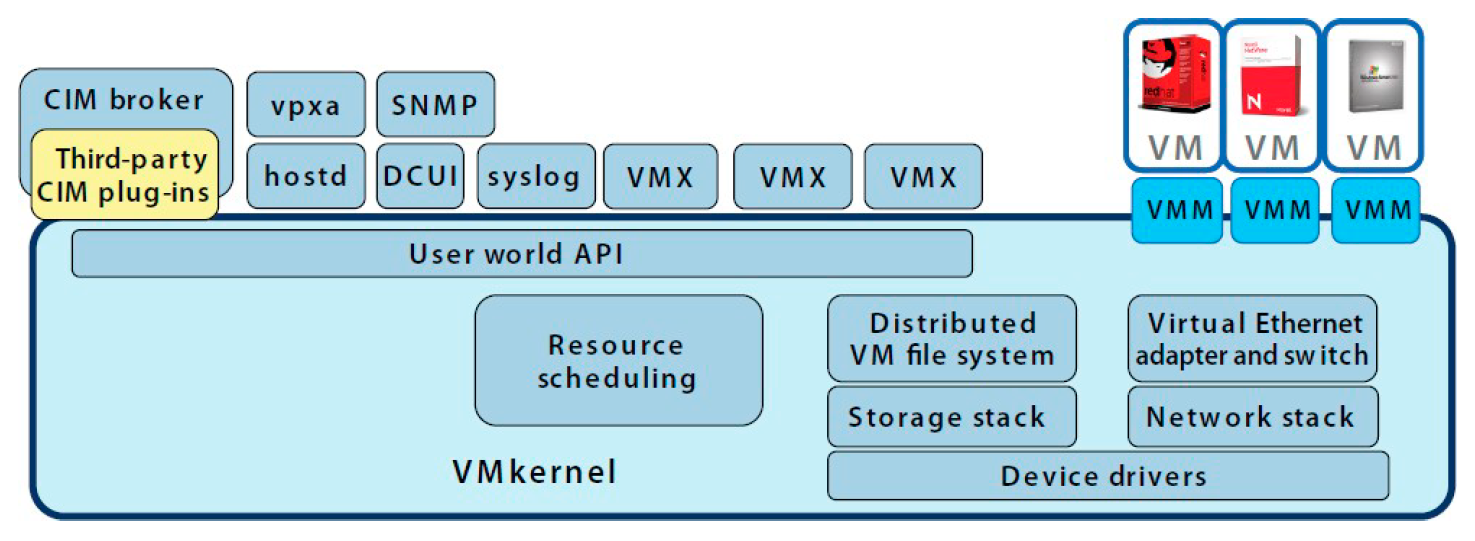
\includegraphics[width=1\textwidth]{imgs/2.1.png}}
    \caption*{\textit{\href{http://plone.4aero.com/Members/lmarzke/talks/vmug_esxi/esi_architecure_steamlined.png/image}{Архитектура гипервизора ESXi}}}
    \label{framework} %framework,fig1
\end{figure}

Будучи одним из ранних гипервизоров, VMware ESXi был выполнен в виде монолита: ядро, все
службы, драйверы устройств, диспетчер памяти собраны в единый, исполняемый в одном адресном
пространстве, модуль. Это, с одной стороны, самое простое и эффективное решение с точки зрения
взаимодействия между компонентами гипервизора. С другой стороны, при таком подходе возникают
некоторые, скажем так, особенности.

\begin{enumerate}
    \item \textbf{Поддерживается ограниченный набор оборудования}. То есть для запуска данного
    гипервизора требуется иметь сервер в жёстко регламентированной конфигурации. Процессор,
    набор системной логики, сетевая карта и накопитель данных — всё должно быть в списке
    поддерживаемой аппаратуры. Для удобства пользователей есть специальная база данных с
    возможностью поиска под названием \href{https://www.vmware.com/resources/compatibility/search.php}{VMware Compatibility Guide}.
\end{enumerate}

Несмотря на видимую строгость условия, возможно добавление некоторых дополнительных
драйверов в установочный образ VMware ESXi, что несколько увеличивает парк совместимой
аппаратуры. Пожалуй, самый простой и доступный вариант — это микрокомпьютеры Intel NUC с
процессорами Intel Core. Но и в случае с Intel NUC следует предварительно поискать информацию об
успешном использовании гипервизора VMware ESXi на данной модели компьютера.

\begin{enumerate}
    \item[2.] \textbf{Небогатый набор инструментария для управления гипервизором}. По умолчанию
    доступны лишь веб-интерфейс, рудиментарная панель управления в текстовом режиме и
    простенькая командная консоль.
    \item[3.] \textbf{Большая поверхность атаки}. Раз весь код гипервизора работает в самом
    привилегированном режиме, то брешь в безопасности любой части гипервизора фактически
    компрометирует весь гипервизор целиком.
\end{enumerate}

Как показало время, такой дизайн гипервизора вполне жизнеспособен, может быть успешно
использован на огромном числе серверов, продолжать развиваться и всё ещё оставаться более
быстрым и эффективным решением, чем некоторые более современные его собратья.\\

\subsection*{Установка гипервизора}
\addcontentsline{toc}{subsection}{Установка гипервизора}

Как мы помним, гипервизор VMware ESXi самостоятельно реализует взаимодействие со всей
поддерживаемой аппаратурой, перечень которой весьма ограничен. Поэтому установка данного
гипервизора возможна только на некоторые серверы. Эта особенность не позволяет даже для
ознакомительных нужд использовать первый попавшийся компьютер или сервер, если он не состоит
из поддерживаемых компонентов. Остаётся только два варианта: использовать поддерживаемую
конфигурацию или запустить гипервизор внутри виртуальной машины.

Разумеется, это плохая идея для использования гипервизора в полноценном рабочем режиме, однако
для ознакомления с самим гипервизором и интерфейсами его управления это вполне подходящее
решение.

Гипервизор VMware ESXi поставляется в виде ISO-образа загрузочного диска и доступен на веб-сaйте
VMware. После несложной регистрации можно загрузить установочный образ гипервизора для
личного использования с некоторыми ограничениями.

Доступные возможности гипервизора зависят от типа используемой лицензии. Без регистрации
номера лицензии первые 60 дней доступны все функции без исключения. По прошествии 60 дней
необходимо указать лицензию, в противном случае гипервизор продолжит свою работу, но перестанут
действовать дополнительные функции, недоступные в бесплатной версии, и остановленные
виртуальные машины будет невозможно запустить. Поэтому даже для продолжения использования
гипервизора в его бесплатной версии необходимо получить на сайте VMware бесплатную лицензию и
зарегистрировать её в гипервизоре.

Из важных ограничений бесплатной версии стоит отметить невозможность управления гипервизором
из VMware vCenter, а также отсутствие какой бы то ни было поддержки от VMware Support. Есть и
другие ограничения, однако всё ещё возможно запускать неограниченное количество гостевых систем
и физической памяти, использовать все имеющиеся физические ядра хозяйской системы. То есть
доступен вполне достаточный арсенал для обучения и практики, не требующий финансовых затрат.

ISO-образ диска необходимо разместить на внешнем накопителе: записать на CD/DVD или при
помощи специального ПО, например \href{https://unetbootin.github.io/}{UNetbootin}, создать из этого образа загрузочный
USB-накопитель. Да-да, образ размером чуть более 300 Мбайт всё ещё можно разместить на старом
добром компакт-диске, имеющем обычно полезный объем порядка 600 Мбайт.

Затем можно загрузиться с подготовленного носителя и пройти несколько шагов в интерфейсе
установщика. Важно выбрать накопитель для установки самого гипервизора, причём очень
желательно, чтобы этот накопитель был отдельным физическим устройством, которое не будет
использоваться для хранения гостевых систем и их данных. Отличный выбор — SD-карта или
USB-накопитель объёмом от 4 Гбайт. Использование небольших внешних накопителей для установки
на них данного гипервизора — это норма даже в серьёзных дата-центрах. Такие накопители
рекомендуются производителями серверов наравне с обычными дисковыми или твердотельными
приводами.

Несколько минут, и система готова к работе. После окончания работы установщика достаточно просто
перезагрузить машину.

\begin{figure}[h]%current location
    \centering
    \scalebox{0.9}{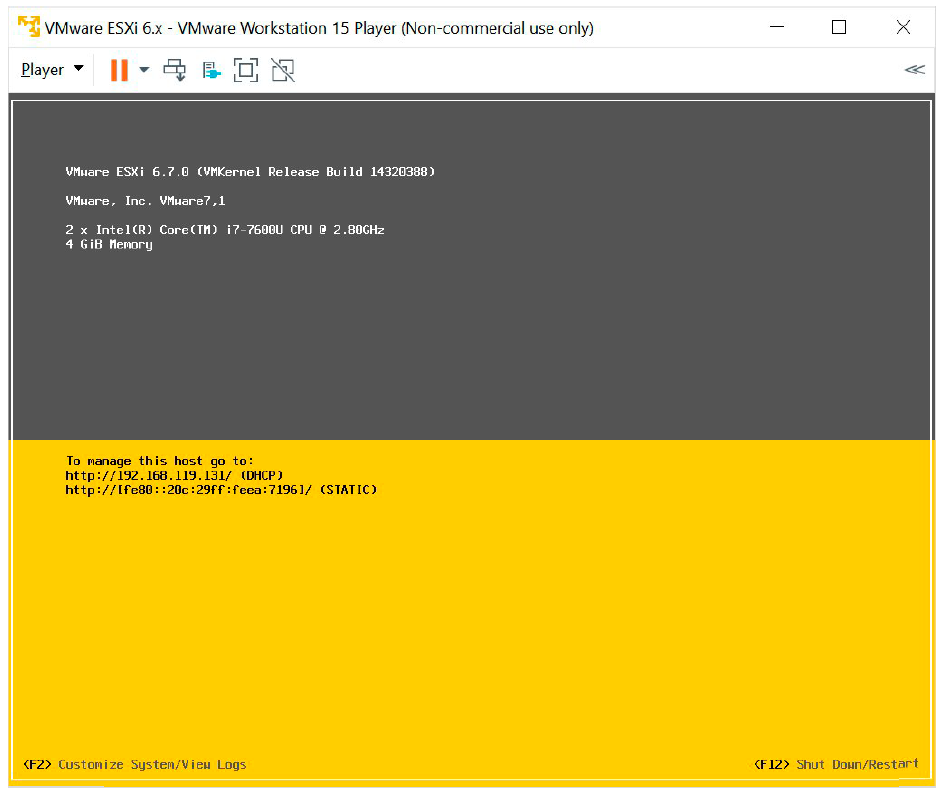
\includegraphics[width=1\textwidth]{imgs/2.2.png}}
\end{figure}

Важное замечание: в конце процесса установки потребуется задать пароль администратора
(пользователя root). Стоит подойти к этому вопросу ответственно и запомнить пароль. В противном
случае не удастся войти в интерфейс управления гипервизором: ни в локальный, ни в его веб-версию.
Проделав описанные выше шаги, мы получим гипервизор, загружающийся с локального накопителя
данных. В терминологии VMware это называется local boot, «местная загрузка».

Будучи зрелым и современным гипервизором, предназначенным для использования в сложных
дата-центрах, гипервизор ESXi может быть использован с гораздо большим количеством сценариев:
stateless, stateless caching, stateful или boot from SAN.

Stateless boot — это техника использования серверов таким образом, когда на самих серверах не
сохраняется никакого промежуточного состояния (stateless — «без состояний»). Данный режим был
представлен в VMware vSphere 5. То есть сервер загружается при помощи PXE, используя сеть. При
этом данные о PXE-сервере поступают от DHCP-сервера, а затем с PXE-сервера образ гипервизора
скачивается в память сервера, и начинается его выполнение.

После старта гипервизора все настройки для данного сервера поступают от центра управления
VMware vCenter Server. Получается, что более не нужно использовать даже SD-карты или
USB-накопители. Кроме того, такой метод загрузки позволяет запросто обновлять используемый на
оборудовании гипервизор. Достаточно лишь перезагрузить сервер и выдать ему для загрузки с
PXE-сервера новую версию гипервизора.

\href{https://ru.wikipedia.org/wiki/PXE}{PXE} (сокр. от англ. Preboot eXecution Environment, произносится «пикси») — среда для загрузки
компьютера с помощью сетевой карты без использования локальных носителей данных (жёсткого
диска, USB-накопителя и т. п.).

\textbf{Stateless caching boot} — по сути, то же, что и stateless, описанный ранее, но при получении нового
образа гипервизора он сохраняется на локальном накопителе. Преимущество этого режима состоит в
том, что система всё ещё сможет стартовать с локального накопителя, если серверы DHCP, TFTP или
Auto Deploy окажутся неработоспособны или недоступны. Однако есть и несколько неприятных
особенностей, которые стоит иметь в виду. Во-первых, нужно позаботиться о наличии локального
накопителя, который будет использоваться только для хранения образа гипервизора. К сожалению,
использовать часть диска, предназначенного для хранения данных (если таковой в системе уже есть),
нельзя. Во-вторых, сохранённая локально версия гипервизора может оказаться устаревшей, если
версия гипервизора, раздаваемая сервером Auto Deploy, была обновлена.

\textbf{Stateful boot} или даже \textbf{stateful installation} — крайний случай stateless caching boot, при котором
образ гипервизора загружается и устанавливается на локальный диск, и впоследствии система всегда
использует локально установленный гипервизор для загрузки. Имеет те же недостатки, что и stateless
caching.

Все три перечисленных выше режима загрузки были представлены в VMware vSphere 5. Для их
реализации рекомендуется использовать VMware vSphere Auto Deploy.

\subsection*{Использование гипервизора}
\addcontentsline{toc}{subsection}{Использование гипервизора}

При включении хозяйской системы происходит загрузка гипервизора: стартует ядро VMkernel,
инициализируются драйвера устройств, система логирования и интерфейсы управления. Образ
гипервизора может загружаться с локального диска или по сети.

Первый интерфейс, называемый Direct Console DCUI (Direct Console User Interface), доступен
локальному администратору при непосредственной работе с сервером при помощи монитора и
клавиатуры. В нём можно выполнить самые простые и критические настройки: задать или изменить
пароль пользователя, проверить и/или изменить сетевые настройки, включить доступ по SSH или,
наконец, сбросить все настройки до значений по умолчанию. По умолчанию доступ по SSH закрыт в
целях повышения безопасности.

\begin{figure}[h]%current location
    \centering
    \scalebox{0.9}{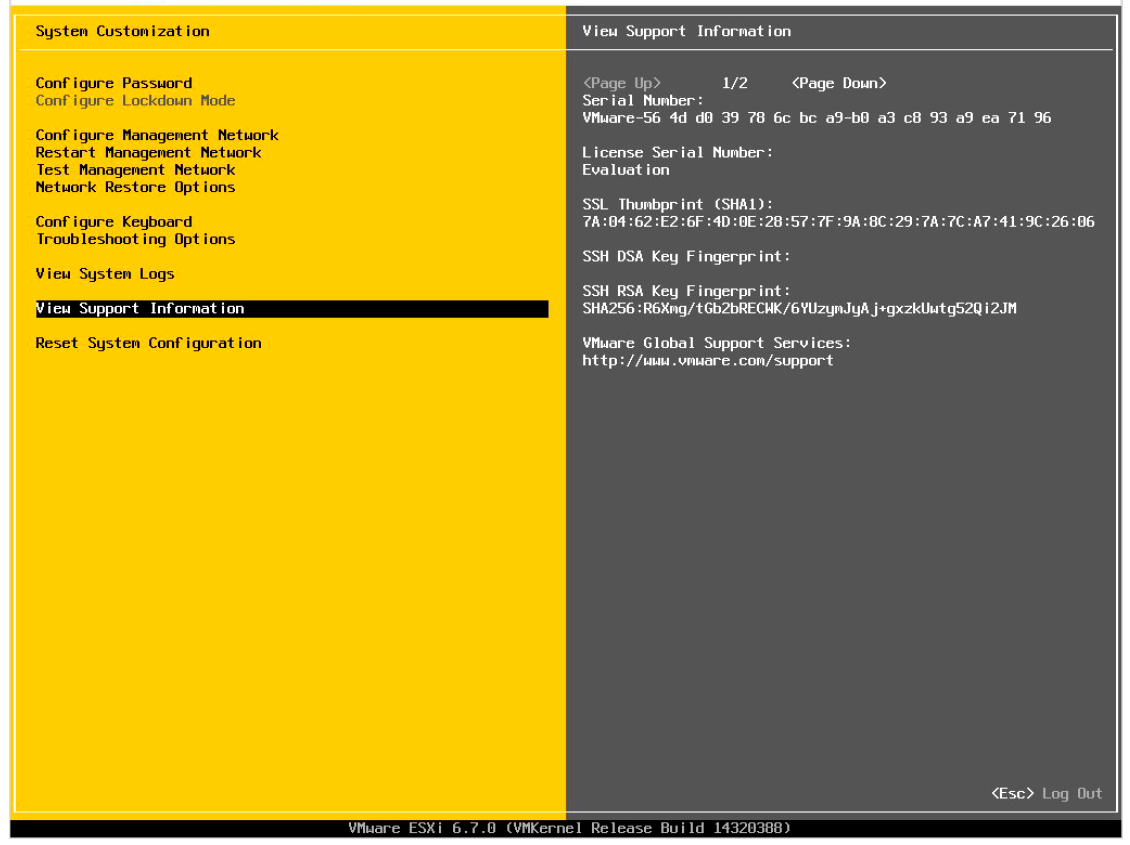
\includegraphics[width=1\textwidth]{imgs/2.3.png}}
    \label{framework} %framework,fig1
\end{figure}

Дополнительно, при \href{https://vmblog.ru/kak-vklyuchit-ssh-v-vmware-esxi-6-x/}{включении доступа через SSH}, становится доступен интерфейс ESXi Shell. По
сути, это сильно модифицированная UNIX-подобная командная консоль, которая позволяет
производить огромное количество разнообразных манипуляций с самим гипервизором и
виртуальными машинами, запущенными поверх него.

\begin{lstlisting}
# ssh root@192.168.119.131

The time and date of this login have been sent to the system logs.

WARNING:
   All commands run on the ESXi shell are logged and may be included in 
   support bundles. Do not provide passwords directly on the command line.
   Most tools can prompt for secrets or accept them from standard input.
    
VMware offers supported, powerful system administration tools. Please see
www.vmware.com/go/sysadmintools for details.

The ESXi Shell can be disabled by an administrative user. See the vSphere
Security documentation for more information.

[root@localhost:~] uname -a
VMkernel localhost.localdomain 6.7.0 #1 SMP Release build-14320388 Aug 5
2019 02:37:06 x86_64 x86_64 x86_64 ESXi
\end{lstlisting}

Более того, подключившись к ESXi Shell через SSH, можно запустить DCUI и работать с ним удалённо.
Смотрите инструкцию в \href{https://docs.vmware.com/en/VMware-vSphere/6.7/com.vmware.vsphere.security.doc/GUID-94F0C54F-05E3-4E16-8027-0280B9ED1009.html}{Use the Direct Console User Interface (DCUI) to Enable Access to the ESXi Shell}.

Одно важное замечание: необходимо установить переменную окружения TERM=linux в SSH клиенте,
в противном случае DCUI молчаливо не будет запускаться.

\begin{figure}[h]%current location
    \centering
    \scalebox{0.8}{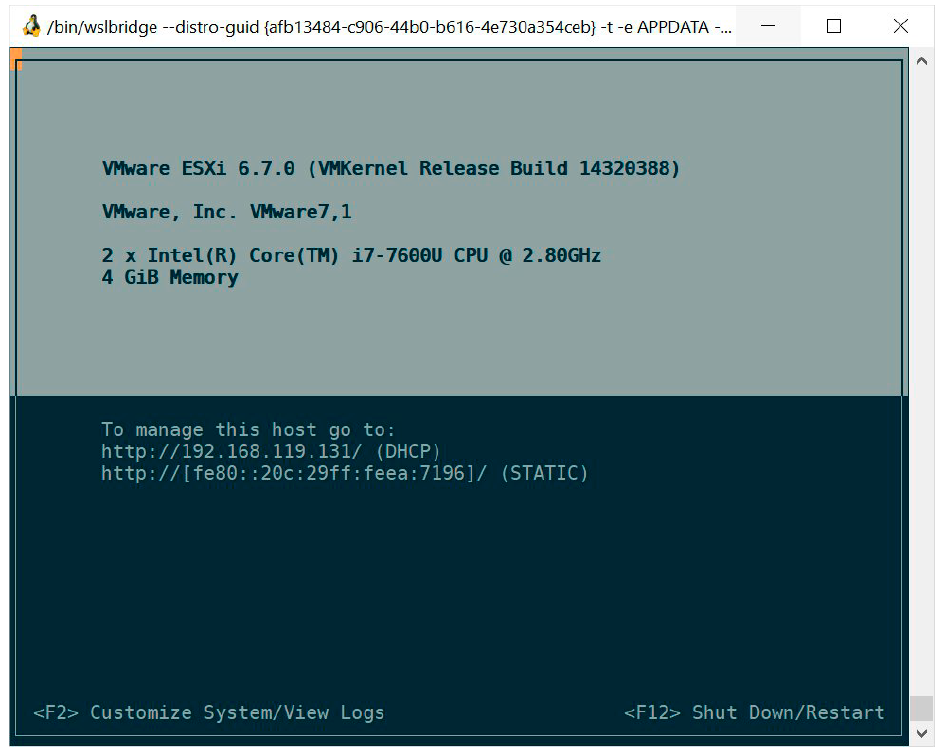
\includegraphics[width=1\textwidth]{imgs/2.4.png}}
    \label{framework} %framework,fig1
\end{figure}

Гораздо более наглядный и удобный интерфейс управления доступен при помощи браузера. В нём
можно управлять гипервизором, создавать и настраивать виртуальные машины, изучать логи и т. д.
Кроме того, информация о состоянии аппаратуры и гостевых систем представлена в том числе в виде
графиков, что позволяет с первого взгляда оценить состояние всей системы в целом.

\begin{figure}[h]%current location
    \centering
    \scalebox{1}{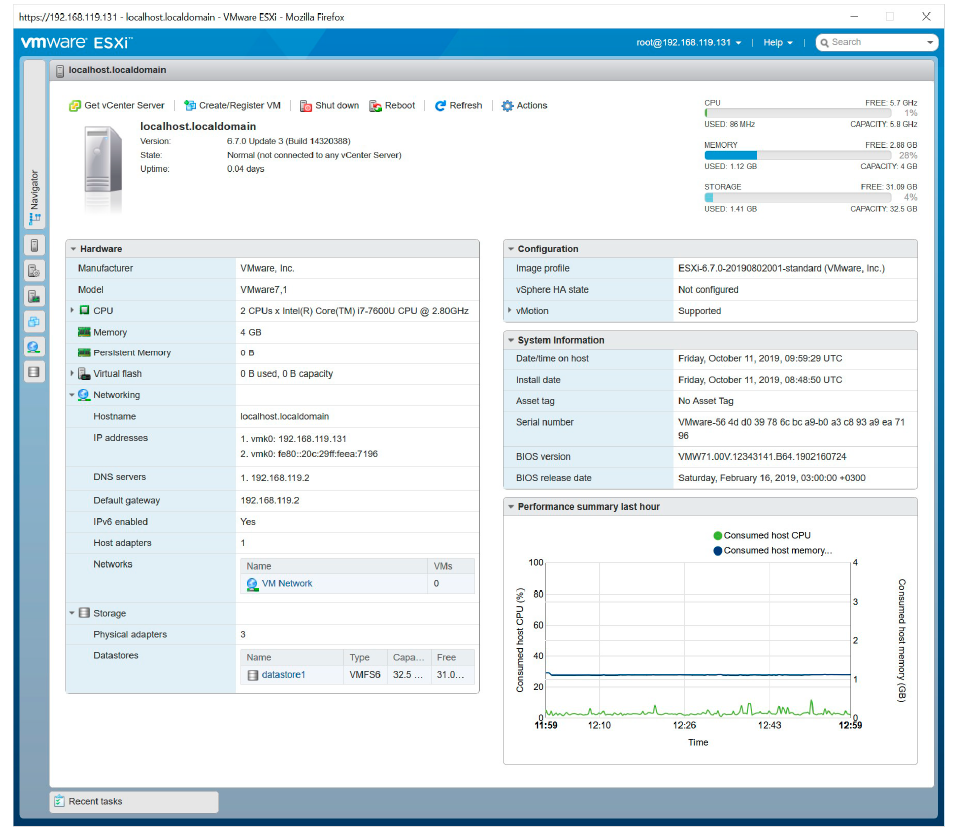
\includegraphics[width=1\textwidth]{imgs/2.5.png}}
    \label{картинка 2.5} %framework,fig1
\end{figure}

\subsection*{Создание виртуальных машин и управление ими}
\addcontentsline{toc}{subsection}{Создание виртуальных машин и управление ими}

Как и в случае установки самого гипервизора, создание виртуальных машин и управление ими может
быть выполнено вручную пользователем или автоматически сервером vCenter.

Пользователь может создавать виртуальные машины достаточно разнообразными методами:

\begin{enumerate}
    \item Создание совершенно новой конфигурации виртуальной машины по шагам в веб-интерфейсе
    гипервизора.
    \item Создание виртуальной машины из имеющегося шаблона.
    \item Создание клона уже имеющейся виртуальной машины.
\end{enumerate}

Причём последние два метода доступны при помощи веб-интерфейса самого гипервизора и
веб-интерфейса сервера vCenter.

Помимо создания виртуальной машины, возможен импорт предварительно созданной, в том числе из
OVF- или OVA-образов.

\href{https://ru.wikipedia.org/wiki/Open_Virtualization_Format}{OVF} (сокр. от англ. Open Virtualization Format) — открытый стандарт для хранения и распространения
виртуальных машин. Стандарт описывает открытый, переносимый, расширяемый формат для
распространения образов виртуальных машин. Стандарт OVF не привязан к какой-либо реализации
гипервизора или аппаратной архитектуре.

Подробную инструкцию можно найти в документации VMware: \href{https://docs.vmware.com/en/VMware-vSphere/6.7/com.vmware.vsphere.vm_admin.doc/GUID-39D19B2B-A11C-42AE-AC80-DDA8682AB42C.html}{Deploying Virtual Machines}.\\

\subsection*{Работа под управлением сервера централизованного управления vSphere}
\addcontentsline{toc}{subsection}{Работа под управлением сервера централизованного управления vSphere}

Гипервизор VMware ESXi находит наиболее частое применение в сложных вычислительных
кластерах, где ручное управление гипервизором и отдельными виртуальными машинами
неэффективно. А потому, как правило, всей этой сложной системой управляет сервер VMware vCenter
Server, особенности которого мы рассмотрим позднее, когда будем говорить о системах управления
виртуализацией.\newpage

\section*{Резюме}
\addcontentsline{toc}{section}{Резюме}

Рассмотрев только основные возможности гипервизора VMware ESXi, можно сделать вывод, что это
мощный и гибкий инструмент для построения сложных систем серверной виртуализации. Судя по
тому, что значительная часть рынка серверной виртуализации (особенно если говорить о крупных
корпоративных пользователях) использует именно продукты VMware и именно VMware до сих пор
продолжает создавать и продвигать на рынок новые и всё более интересные решения, связанные с
виртуализацией, можно смело назвать компанию VMware лидером на этом рынке.\\


\section*{Используемые источники}
\addcontentsline{toc}{section}{Используемые источники}

\begin{enumerate}
    \item \href{https://www.us-cert.gov/sites/default/files/publications/data_backup_options.pdf}{Data Backup Options, Paul Ruggiero and Matthew A. Heckathorn, United States Computer
    Emergency Readiness Team}
    \item \href{https://www.simongreaves.co.uk/understand-auto-deploy/}{VMware How To: Understand Auto Deploy – vSphere 6.7, Simon Greaves}
\end{enumerate}

\section*{Практическое задание}
\addcontentsline{toc}{section}{Практическое задание}

\begin{enumerate}
    \item Какими преимуществами и недостатками обладают гипервизоры первого типа по сравнению с
    гипервизорами второго типа?
    \item Благодаря чему гипервизоры первого типа оказываются более эффективными, чем
    гипервизоры второго типа?
    \item * Установите гипервизор VMware ESXi на доступный компьютер или виртуальную машину и
    выполните измерения производительности основной ОС и такой же ОС, установленной в
    гипервизоре.
\end{enumerate}

\href{https://www.phoronix-test-suite.com/}{Phoronix Test Suite} — удобный и мощный инструмент для запуска разнообразных тестов.

\end{document}